
\section{The Proposed Approach}
\label{sec:approach}

In this section, we describe the proposed approach, which utilizes
an item-based recommender system to improve test case prioritization techniques. 
Figure~\ref{fig:workflow} shows three major activities in our approach and
how these activities are related to each other. 
The first step of our proposed technique is usage pattern extraction, 
which is shown in the upper box of the Figure~\ref{fig:workflow}. 
In this activity, we analyze the users' interaction data to 
determine the most frequently accessed components of the system. 
Our second activity is change history analysis, which is shown in the
lower box of the Figure~\ref{fig:workflow}. In this activity,  
we build a classification model to 
measure the relationship between software defects and change history metrics. 
Then, by obtaining the output from these two activities, we measure the risk 
score of each component and prioritize the test cases based on their coverage
of these risky components. In this paper, component refers to method. 

\begin{figure*}[!hb]
\vspace*{-12pt}
	\centering
	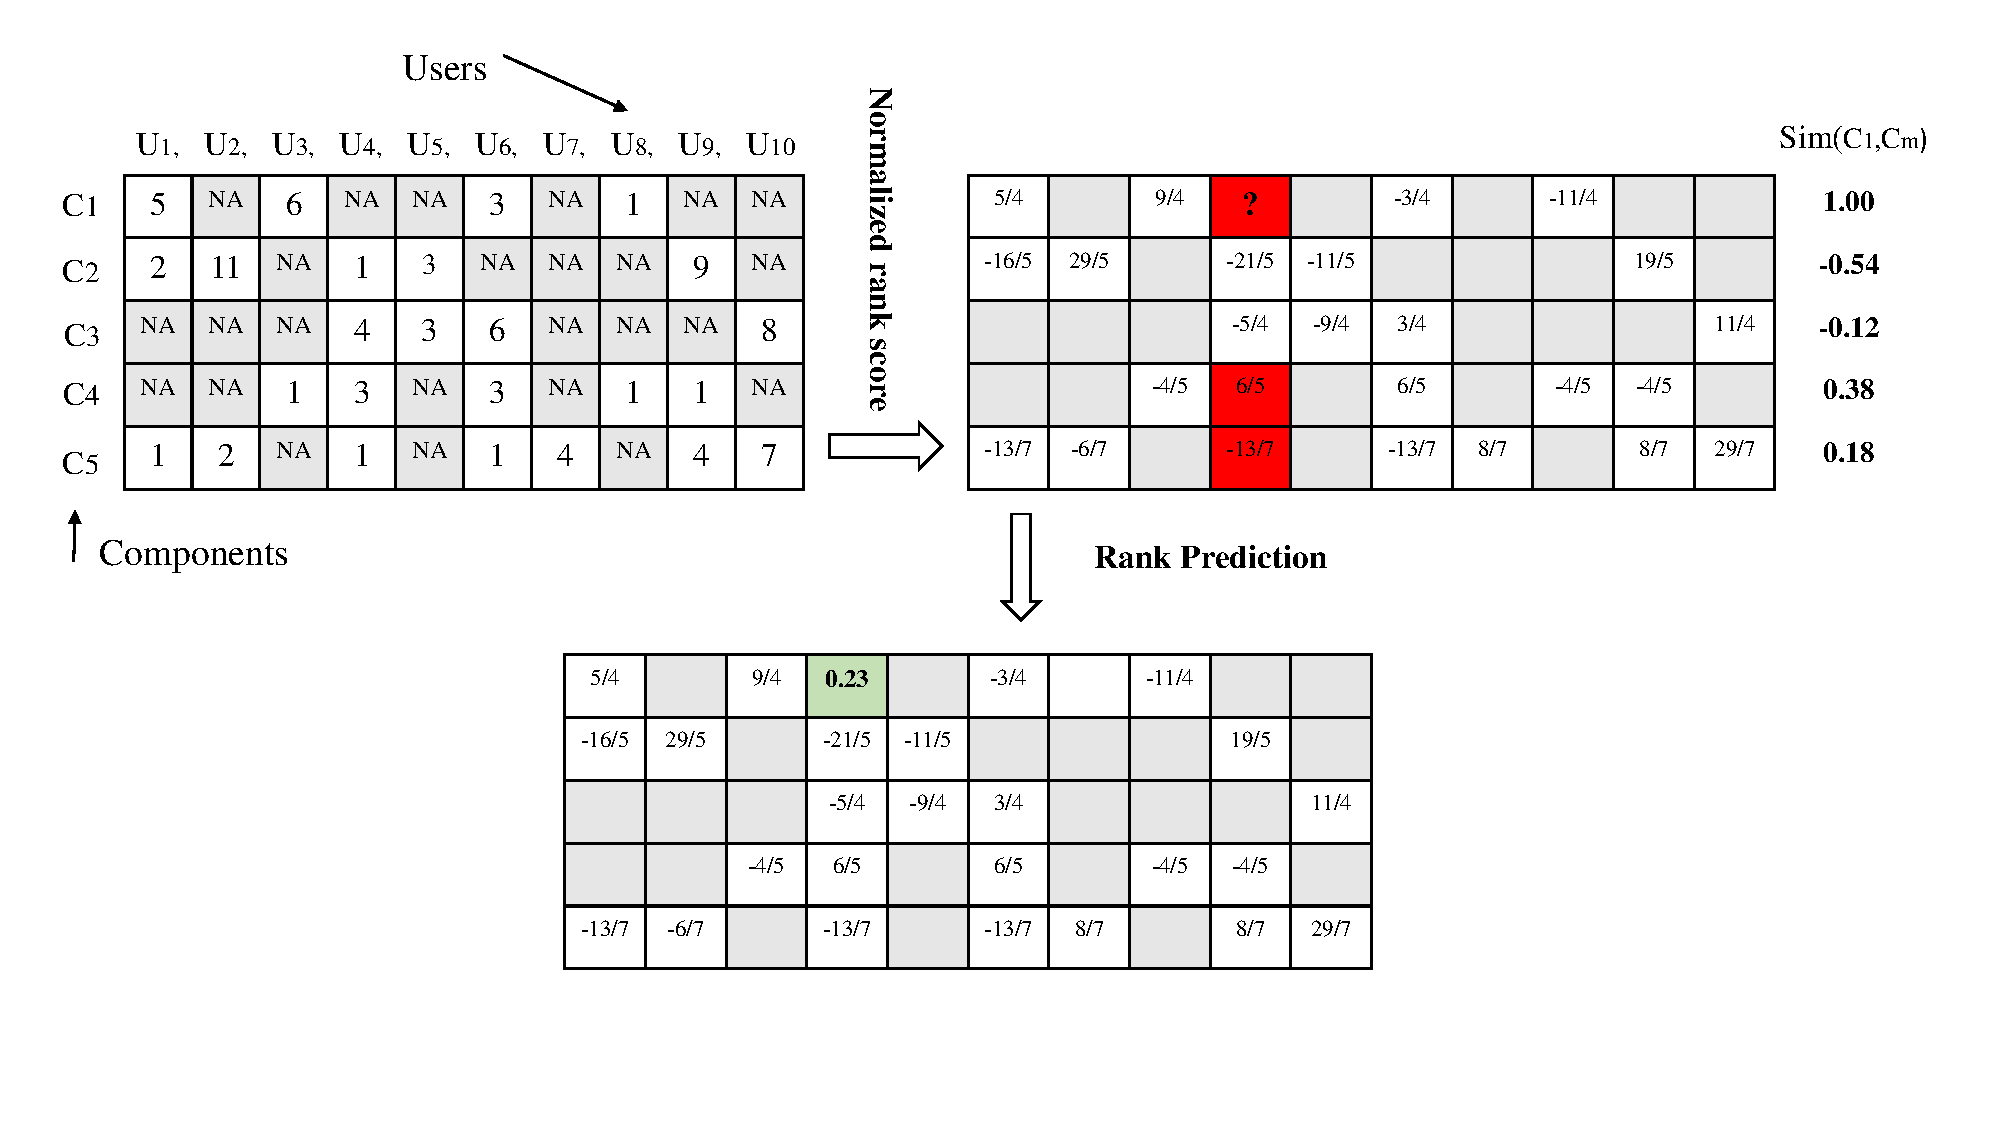
\includegraphics[width=0.8\linewidth]{./collaborative-filtring22.pdf}
\vspace*{-30pt}
	\caption{Item-Based Collaborative Filtering Process for Identifying Most-Frequent Components}
	\label{fig:collaborataivefiltering}
\end{figure*} 

\subsection{Usage Pattern Extraction}
\label{recommender-approach}

The goal of our recommender system is to suggest the highest-risk 
components with the most access frequency among all other components in the applications. 
In large scale applications, there are wide range of features and components; 
however, in reality, only a relatively small subset of components is accessed by users. 
Therefore, even if there are bugs in some part of the system that is not generally access by  users, we assume that those bugs have less impact on the user-reliability perception
of a system; catching those bugs that have been exposed by users is a bigger priority.
Also, prioritizing the test cases that exercise these more
frequently accessed components can speed up the rate of fault detection. 
 
There are two primary techniques for collaborative filtering algorithms:
user-based and item-based algorithms. 
A user-based collaboration filtering algorithm tries to find 
users who are most similar to the current active user.
In an item-based algorithm, first we design a model of user rating, 
and then we evaluate the expected ratings of an item based on the previous 
ratings of the other similar items. Because our concern is to find the 
access frequency of the components rather than user preferences, 
we chose an item-based algorithm.

To calculate the access frequency of the components,
we used two collected data sets: 
a list of users $U=\{u_1, u_2, ..., u_m\}$ and 
a list of the components $C =\{c_1, c_2, ..., c_n\}$. 
Each component $c_i$  has a list of users' ratings if 
users have performed at least one task with it.
Typically, in recommender systems, prediction is based on the numerical values of 
ratings from active users, but in our case we do not have access to such rating 
modules; instead, we refer the value of access frequency for a specific component 
by an individual active user as a rating score. 

Suppose that a user has interacted with a set of components,
$\{c_1, c_2,$ $..., c_n\}$. 
The item-based collaborative algorithm
computes the similarity between components by calculating the cosine similarity 
of the ratings of two components. 
Then, the algorithm selects the $N$ most similar components 
%$\{c_1, c_2, ..., c_N\}$ 
that has the highest similarity score to $c_i$.
%We defined the set of $k$ most similar components as $N$.
%Further, corresponding similarities $\{s_{i1}, s_{i2}, ..., s_{ik}\}$  
%between components are also estimated. 

After finding the components that have the highest similarity score, 
we need to predict the ratings of those
components that have been ignored or have not yet been used.
To do this, the algorithm uses a weighted average of the target user ratings
on these similar components.
Below, we describe the process of computing similarity and ranking.

Suppose that we have a web application that has several functionalities; 
a group of users shows similar interests in using a set of components,
while other groups of users use different sets of components. 
We want to measure the similarity between components by considering users' activities 
and their preferences in using the components.
 
Figure~\ref{fig:collaborataivefiltering} illustrates an example of
component similarity prediction. The upper left-hand matrix in the figure shows 
how many times each component has been used by users. 
The numbers in the cells show the access frequency by the
user $u_{i}$ on the component $c_{j}$, 
and $NA$ indicates that the user $u_{i}$ has not used that 
particular component yet. In this figure, $u_{1}$, $u_{3}$, $u_{6}$, and $u_{8}$ 
utilized components $c_{1}$; and $u_{1}$, $u_{2}$, $u_{4}$, $u_{5}$, and $u_{9}$ 
utilized $c_{2}$. 
We refer to a set of component ratings as a component vector.
For example, the vector $c_1$ is $\{5, NA, 6, NA, NA, 3, NA, 1, NA, NA\}$. 
Once we identify the component vectors, we measure the similarity 
between $c_{i}$ and all other components one by one. 

In order to determine the similarity between two components $i$ and $j$, we use
Pearson-r correlation~\cite{recom}.
If $U$ is the set of users who rated components $i$ and $j$, then we compute
the correlation similarity using the following equation:

\vspace*{-3pt}
\[
{Sim (i,j) = \frac {\sum_{u\in {U}}(C_{u,i} - \bar{C_i})(C_{u,j} - \bar{C_j)}}
	{ \sqrt{\sum_{u\in {U}}({C_{u,i} - \bar{C_i}})^{2}}
		{ \sqrt{\sum_{u\in {U}}({C_{u,j} - \bar{C_j}})^{2}}}}}	
\]

where $C_{u,i}$ is the value of access frequency for component $i$ by user $u$, and
$\bar{C_i}$ is the average access frequency value of $C_i$ . 

The reason for finding the similarity between components is to find the missing 
value in the matrix. To measure the similarity between components, 
we normalize the rating of each component by subtracting the row mean. 
The upper right-hand matrix in Figure~\ref{fig:collaborataivefiltering} shows the normalized
rating values of the left matrix. 
For example, the average of access frequency of $c_{1}$ and $c_{2}$  is $15/4$ and $26/5$, respectively.
Then, we subtracted mean values from each corresponding row of the left matrix.  
Positive values indicate that the user liked the component more than average;
while negative values
indicate that the user liked the component less than average; 0 indicates the average access 
frequency for a component. 
We treat blank values as 0.
The rightmost column in the upper right-hand matrix shows the similarity 
between $c_{1}$ and all other
components. For example, $Sim(c_{1},c_{2})= -0.54 < Sim(c_{1},c_{4})= 0.38$ means
that the probability of rating of $c_{1}$ is much more like $c_{4}$ than $c_{2}$.  

After calculating the similarity between all components, we select 
the set of $N$ most similar components for $c_{i}$;  
this process will be iterated for every component. 
Once we have this set of $N$, then we can make a prediction of access frequency 
for the missing values of $c_{i}$ based on a rating of the $N$ similar components.
To estimate the access frequency rates of ignored components, we performed
ratio prediction computation using a weighted sum method.
This method provides the ratio prediction of a specific component $i$
for user $u$ based on similar components. 

\vspace*{-3pt}
\[
{P_{u,i} = \frac {\sum_{{all\: simillar\: components , N}}(S_{i,N} * R_{u,N})}
	{\sum_{{all\: simillar\: components, N}}({S_{i,N}})}}
\]

$R_{u,N}$ is the rating score for user $u$ and $N$ most similar components, 
and $S_{i,N}$ is the similarity score of component $i$ and $N$.

We illustrate this using an example in Figure~\ref{fig:collaborataivefiltering}.
The lower matrix in the figure shows the predicted frequency access for $P_{1,4}$, 
which is calculated by $(0.38 * 6/5 + 0.18 * -13/7) / (0.38 + 0.18) = 0.23$.   

The number, $N$, is determined based on the context of application domain, 
ranging from 1 to size of $C - 1$. 
However, assigning a large number to 
$N$ will increase the calculation cost significantly, while the result accuracy would not
change noticeably. Therefore, to reduce the cost of the calculation process, 
we set $N=2$ , 
which means that to predict the missing values we only
select the two most similar components to $c_i$. 
This process is repeated until we find the ranking for the all missing values. 
Once we calculate ratio scores for the components, we can produce a matrix of components
and their access frequency ranking scores.  
We calculate normalized access frequency scores
using the following equation:

\[
{F_{Ci} = \frac {{\sum}(P_{Ci})}
	{{number\: of\: components}}}
\]

where $P_{Ci}$ is the predicted rank score and $F_{Ci}$ is the
normalized rank score of component $i$. 
Then we can sort the matrix of components based on their ranking to 
select $Top-N$  most frequently accessed components.

\vspace*{-3pt}
\subsection{Change History Analysis}
\label{CIA-approach}
\vspace*{-2pt}

The second phase of our proposed approach is change history analysis.
Among hundreds of attributes of code and change history metrics to evaluate
the code quality and error proneness, we chose change history metrics to identify
the riskiest components. According to a previous study~\cite{raimund},
change history is a better indicator for bug prediction purposes than code metrics.
 

The process of change analysis involves two major steps. 
First, we collect change history information (e.g., added lines of code,
deleted lines of code, etc.) and bug reports
from all available versions of the
applications from their repositories.  
The details of collecting the change history information 
are discussed in Section~\ref{data-collection}.  
Once the change history data is collected, 
we then design a linear model from a set of collected 
change metrics to build a classification model for bug prediction.
Our goal is to find the correlation coefficient of each 
metric to measure statistical relationships between a change metric and 
real defects. 
The value of this measure 
ranges between 1 and -1, where 1 indicates a strong 
positive relationship, 0 indicates no correlation, and a
negative value indicates a reverse correlation.

To evaluate our linear model, we applied 10-fold cross validation
and repeated this process 100 times. 
We used a common accuracy indicator to determine the accuracy of 
our model. 
%Table~\ref{tab:ConfusionMatrix} shows the confusion matrix that we used
%for accuracy evaluation.
The three accuracy indicators that we used are PC, TP and FP. 
PC indicates the percentage of correctly classified 
instances,
% which is calculated using $(m_{11} + m_{22})/(m) * 100\% $. 
TP (true positive) indicates the number of components
that contain a bug (and our classification
model also classified them as buggy components), 
%which is obtained by $m_{22}/(m_{22} + m_{21})$,
and FP (false positive) is the number of components that 
are classified as buggy (but they are clean). 
%which is calculated by $m-{12}/(m_{12}+m_{11})$ . 
%A higher PC value means that our classifier model is effective. 
The output of our classification model is a list of components with
their risk values, $I_{Ci}$ (the risk score of being buggy for component $i$).

%\begin{table}[!ht]
%	\caption{Confusion Matrix}
%	\vspace*{-10pt}
%	\begin{center}
%		\begin{tabular}{|l||c||c||c|}
%			\hline
%			Metrics     & Predicted: No & Predicted: Yes &  \\ \hline
%			Actual: No  &     $m_{11}$ = 33   &     $m_{12}$ =  63   & $m_1$ = 96 \\ \hline
%			Actual: Yes &     $n_{21}$ = 54   &     $m_{22}$ =  46   & $m_2$ = 100 \\ \hline
%			&      87       &       109      & $m$ = 196 \\ \hline
%		\end{tabular}
%		\end {center}
%		\label{tab:ConfusionMatrix}
%		\vspace*{-5pt}
%\end{table}
	
%A higher PC value means that our classifier model is effective 
%If PC is high but the recall (TP) low, this means that our classifier 
%classified a large number of components as clean when they are not, 
%indicating that we missed many buggy component during this phase
%of testing. However, if FP is high, this indicates that our model detected many components as buggy when they 
%are clean, and this will add extra cost to test the system when such a cost is not warranted. 
%The output of our classification model is a list of components with
%their risk values, $I_{Ci}$ (the risk score of being buggy for component $i$).

\vspace*{-3pt}
\subsection{Test Prioritization Using the Recommender System}
\label{test-prioritization}

After obtaining the two metrics explained in previous subsections (component risk scores and 
access frequency ratios), we calculate the final risk scores using the following equation:

\vspace*{-3pt}
\[
{ R_{Ci} = F_{Ci} * I_{Ci}}	
\]

\vspace*{-3pt}
where $F_{Ci}$ is the access frequency score of component $i$ 
and $I_{Ci}$ is the fault risk score of $C_i$.  

Using $R_{Ci}$ scores, our recommender system provides a ranked list of components.
The ranked list of components contains those components of the system that are most
likely to be the cause of regression faults. 
As shown in Figure~\ref{fig:workflow}, the test case prioritization algorithm
reads two inputs (a recommended $Top-N$ list of components and code coverage of tests),
and reorders test cases. 

For example, suppose we have five components
$C =\{c_1, c_2, ... , c_5\}$ with risk scores 
$R =\{0.0014, 0.251, 0.034 , 0.561, 0.138\}$.
Also, suppose we have a list of test cases with their code coverage information
, such as $TC =\{T_1 ={(c_5, c_3)}, T_2={c_1}, T_3={(c_4, c_2)}, T_4={(c_2,c_5)} , T_5={c_2}\}$ .
Then, we reorder the test cases in this order:
$T_3, T_4, T_1, T_2, T_5$, 
since $T_3$ covers $c_4, c_2$, the two components 
having the highest risk score (0.561 + 0.251 = 0.812), and $T_2$ and $T_5$ will be
executed last because $T_2$ covers $c_1$, which has the lowest risk score (0.0014).
$T_5$ only covers $c_4$ (this component has been covered by $T_3$ as well); and because 
$T_4$  covers more components (0.251 + 0.138 = 0.389), then it has higher priority than 
$T_5$, which covers only $c_2 = 0.251$.
Finally, we calculate the fault detection rate of the reordered test cases by 
applying the proposed technique in the latest version of each application.  


